\documentclass[../../main.tex]{subfiles}

\begin{document}

\setchapterpreamble[u]{\margintoc}

\chapter{双指针}

双指针是在算法中考察的很多的一类问题,其依赖于两个指针互相移动从而解决问题。
指针的移动方向可以相同,也可以相反,也可以是一前一后,这些都是根据具体问题而定的。

在我看来,这上面的话都是废话。并没有告诉你应该如何去实际的解决一个问题。这个章节主要
就是根据实际的问题来思考该如何使用双指针。

\section{N数和}

\subsection{\href{https://leetcode-cn.com/problems/two-sum/}{两数之和}}

几乎所有解决这个问题的方法都是使用哈希表,但是这里我们使用双指针来解决这个问题。
当我们解决了这个问题,我们才能继续地思考三数之和,四数之和等等问题。

这个题的暴力解法是显而易见的。如果要使用双指针解决这个问题,我们的做法就是排序,
然后使用两个指针分别指向数组的头和尾,然后根据两个指针指向的元素的和与目标值的
大小关系来移动指针。\sidenote{排序加双指针是一种常见的思想,通常用于解决需要在排序数组中找到
满足特定条件的元素对的问题}

在这个过程中,我们可以确定一个循环不变量:\textbf{在数组中,左侧指针之前的所有元素都小于等于
右侧指针之后的所有元素}。对指针\texttt{start}和\texttt{end},我们可以得到其值

$$
sum = nums[start] + nums[end]
$$

如果$sum$小于目标值,那么我们就需要增大$sum$,所以我们需要增大texttt{start},反之亦然。
我们可以简单地写出如下的代码:

\lstinputlisting[language=C++]{code/two_sum.cpp}
\sidenote{上述代码假设数组已经完成了排序}

\subsection{\href{https://leetcode-cn.com/problems/3sum}{三数之和}}

这个问题是上一个问题的升级版,我们需要找到所有的三元组,使得三元组的和为0。我们可以很简单地把这个
问题转化为两数之和的问题,即确定一个数,然后在剩下的数中找到两个数,使得这两个数的和为确定的数的
相反数。这个问题的难点在于如何去除重复的三元组。

首先,我们能够做一个最简单的去重思考。

\begin{example}
  假设$array = [1, -1, -1, -1, 2]$,当我们确定到$-1$时,我们可以得到一个唯一
  的三元组$(-1, -1, 2)$,当我们确定$-1$的下一个元素时,其也是$-1$,那么我们就会
  得到一个重复的三元组$(-1, -1, 2)$。因此我们需要跳过这个元素,直到我们确定的元素
  和上一个元素不一致。
\end{example}

上述的去重是我们不重复考虑一个相同的元素,但是我们还需要考虑一个问题,就是我们在确定两数之和
时,我们需要跳过相同的元素。

\begin{example}
  假设$array = [-2, -2, -2, -1, 0, 1, 2, 2, 2]$,我们套用两数之和的解法,开始时
  $start = 0, end = 8$。我们可以得到第一个解$(-2, 2)$,并且$start = 1, end = 7$,
  我们同时可以得到第二个解$(-2, 2)$,这不是我们想要的,所以我们需要检测下一个\verb|start|
  和下一个\verb|end|,直到值不相同为止。
\end{example}

再确定好这两个去重条件后,我们就可以写出如下的代码:

\lstinputlisting[language=C++]{code/three_sum.cpp}

在这个问题中,最关键的问题在于理解到二数之和和三数之和并没有本质的区别。其核心的思路是一致
的。解决了这个问题你就可以下面解决这个类似的问题。

\href{https://leetcode.cn/problems/3sum-closest/}{最接近的三数之和
}

\subsection{\href{https://leetcode-cn.com/problems/4sum}{四数之和}}

可能已经有聪明的读者已经明白了如何解决四数之和了。一个最简单的做法就是确定一个数,然后使用
使用三数之和的代码,并根据Example 1.1.1的思路去重即可。这是最显而易见的方法。也就是再添加
一个\verb|for|循环处理就行了。

\begin{kaobox}[title=思考]
我们该如何解决$N$数之和的问题呢?实际上一个最简单的做法就是回溯,对于每一个数来说,我们有两个选择,
选或者不选。这样的时间复杂度是$O(2^n)$。这样也是很慢的,最实际的做法是对于$N$数之和先求解$N-1$
数之和,但是这样似乎我们无法写出代码出来,因为似乎要展开不确定的循环。最简单的做法就是利用元编程
来处理。当然也可以修改成递归来处理。
\end{kaobox}

\section{回文串}

回文串问题也是一个典型的双指针运用。

\subsection{\href{https://leetcode-cn.com/problems/valid-palindrome/}{验证回文串}}

验证回文串是一个基础的不能再基础的题目了。我们需要判断一个字符串是否是回文串。我们可以使用两个
指针\verb|start|和\verb|end|,分别指向字符串的头和尾,然后判断两个指针指向的字符是否相同。
对于这个特定的题目我们只需要确定其是数字或者字母即可。我们可以使用\verb|isalnum|函数来进行判断,
从而简单地写出如下的代码:

\lstinputlisting[language=C++]{code/valid_palindrome.cpp}
\sidenote{对于这段代码的循环不变量的理解是相当重要的,显然循环不变量就是$0$到$start$,$end$到$n-1$的
字符都是回文串。}

\begin{kaobox}[title=思考]
  在上述代码中,我们确定的两个指针一个位于头,一个位于尾。我们可以使用不同的循环不变量来解决这个问题。
  即$start$到$end$的字符串都是回文串。这个思路有助于解决后面一些比较复杂的问题。
\end{kaobox}

\subsection{\href{https://leetcode-cn.com/problems/valid-palindrome-ii/}{验证回文串II}}

这个问题是上一个问题的升级版,我们可以删除一个字符,判断是否是回文串。那么重要的是删除哪个字符呢?以及何时
需要删除字符呢?我们仍然维持上面循环不变量的思想,当$s[start] \neq s[end]$时,循环不变量就不满足了。
此时,我们需要进行两个操作:

\begin{itemize}
  \item 删除$s[start]$,然后判断$s[start+1]$到$s[end]$是否是回文串。
  \item 删除$s[end]$,然后判断$s[start]$到$s[end-1]$是否是回文串。
  \item 如果两个都不是回文串,那么就返回\verb|false|,否则返回\verb|true|。
\end{itemize}

\lstinputlisting[language=C++]{code/valid_palindrome_ii.cpp}

\subsection{\href{https://leetcode-cn.com/problems/longest-palindromic-substring/}{最长回文子串}}

严格来说,这个题并不能算双指针。因为要得出其双指针的解法需要很复杂的分析。当然,
网上的解题方法很简单地告诉你从中间不断扩散就能把这个问题解决了。俗称中心扩展算法。
我并不觉得这是正常人解决问题的方式。

对于求解这类最优问题,首先思考的就应该是动态规划。我们首先应该假设我们知道长度为$s$
的字符串其最长回文字串的长度,我们在其末尾添加一个新的字符,能不能得到其最长子回文串\sidenote{
或许觉得这一步也没有逻辑,实际上动态规划的题有一个很重要的步骤就是猜。也就是看能不能猜出
最优子结构。}。通过轻易地判断我们可以明白,这样是求不出来的,因为状态丢失了字符串的信息。

于是我们需要换一个思路,在前面我们提到了一个重要的循环不变量:$start$到$end$的字符串都
是回文串。那么我们可以得出一个重要的结论,如果$s[start - 1] == s[end + 1]$,那么循环
不变量仍然成立。那么我们就可以得出状态转移方程:

$$
dp[start][end] = dp[start - 1][end + 1] \land s[start - 1] == s[end + 1]
$$

然而,我们该怎么写出代码呢?在我看来,解决二维dp,最好的方式仍然是进行画图处理,通过观察画出
的二维矩阵来确定如何设置循环。我们假设$s$的长度为5,即我们需要定义一个$5 \times 5$的矩阵。
\sidenote{
$$
\begin{bmatrix}
T & F & F & F & F \\
  & T & F & F & F \\
  &   & T & F & F \\
  &   &   & T & F \\
  &   &   &   & T
\end{bmatrix}
$$
}
我们可以非常简单地得到一个初始值,当$start == end$时,$dp[start][end] = true$。

我们列举出所有的状态转移过程:

\begin{itemize}
  \item $(4,4)$
  \item $(3,4)$
  \item $(3,3) \rightarrow (2, 4)$
  \item $(2,2) \rightarrow (1, 3) \rightarrow (0, 4)$
  \item $(1,2) \rightarrow (0, 3)$
  \item $(1,1) \rightarrow (0,2)$
  \item $(0,1)$
  \item $(0,0)$
\end{itemize}

上述的转移过程我们可以表示在如下所示的矩阵中。红色代表状态的起始,箭头表示状态转移。

$$
\begin{bmatrix}
  \tikzmarknode{O}{\color{red}T} & \tikzmarknode{N}{\color{red}F} & \tikzmarknode{M}{F} & \tikzmarknode{L}{F} & \tikzmarknode{K}{F} \\
  & \tikzmarknode{J}{\color{red}T} & \tikzmarknode{I}{\color{red}F} & \tikzmarknode{H}{F} & \tikzmarknode{G}{F} \\
  &   & \tikzmarknode{F}{\color{red}T}& \tikzmarknode{E}{\color{red}F} & \tikzmarknode{D}{F} \\
  &   &   & \tikzmarknode{C}{\color{red}T} & \tikzmarknode{B}{\color{red}F} \\
  &   &   &   & \tikzmarknode{A}{\color{red}{T}}
\end{bmatrix}
$$

\begin{tikzpicture}[remember picture, overlay]
  \draw[arrow] (C) -- (D);
  \draw[arrow] (E) -- (G);
  \draw[arrow] (F) -- (H);
  \draw[arrow] (H) -- (K);
  \draw[arrow] (I) -- (L);
  \draw[arrow] (J) -- (M);
\end{tikzpicture}

从上面的状态转移过程我们可以得出如下的过程,设置一个变量为\verb|start|从0或者字符串
的末尾进行循环,每次取$dp[start][start]$和$dp[start][start + 1]$不断扩展。令
$localStart = start, localEnd = start || start + 1$。然后每次循环$localStart$加1,
$localEnd$减1,直到$localStart < 0 \lor localEnd \geq s.size() \lor s[localStart] \neq s[localEnd]$。
于是我们就可以得到下面的代码:

\lstinputlisting[language=C++]{code/longest_palindromic_substring_dp.cpp}

观察上述的代码,你可以发现我们并不需要这个二维矩阵,我们只需要一个变量\verb|previous|即可。
这个变量代表上一次的状态,我们只需要在每次循环的时候把上一次的状态保存下来即可。于是我们可以
得到如下的代码:

\lstinputlisting[language=C++]{code/longest_palindromic_substring_dp_optimized.cpp}

这就是所谓的中心扩展算法。在我看来,这才是理解这个问题的正确方式。我们不可能一开始就想到用指针不断
地从中心向两边扩展,但是我们可以通过画图的方式通过观察状态的转移来得到这个算法。

\subsection{\href{https://leetcode-cn.com/problems/palindromic-substrings/}{回文子串}}

这个问题和上个问题没有任何本质的区别,仍然使用中心扩展算法。

\begin{kaobox}[title=小结]
  关于回文串的题还有许多类型,我们暂时告一段落。
\end{kaobox}

\section{滑动窗口}

对于滑动窗口的问题,最关键的就是确定好窗口的性质,确定好窗口的性质,我们才能确定如何移动窗口。
进而确定循环不变量。

\subsection{\href{https://leetcode.cn/problems/longest-substring-without-repeating-characters/}
{无重复字符的最长子串}}

我们维持两个指针,一个是\texttt{windowStart},另一个是\texttt{windowEnd}。我们不断地移动
\texttt{windowEnd},直到出现重复的字符,然后我们移动\texttt{windowStart},直到重复的字符
消失。可见,我们最关键的是一直维持窗口的性质不变。

\lstinputlisting[language=C++]{code/longest_substring_without_repeating_characters.cpp}

\subsection{\href{https://leetcode.cn/problems/substring-with-concatenation-of-all-words/}
{串联所有单词的子串}}

显然,这个题的窗口是显而易见的。我们的窗口大小始终是保持不变的,然而在整个过程中,我们的窗口需要移动
一个单词的长度。同时,为了遍历所有的子串,我们需要窗口的起始位置从$0$到$words[0].size() - 1$。如下图所示:
我们假设数组的大小为$9$,单词的大小为$3$,那么我们的窗口的起始位置就是$0$到$2$,然后窗口的起始位置
就是$1$到$3$,以此类推,直到窗口的起始位置为$6$到$8$。然后我们改变窗口的起始位置到$1$,继续重复
上面的步骤。

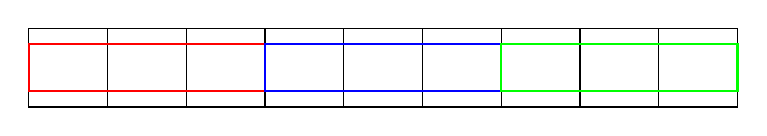
\begin{tikzpicture}
  % draw the array
  \foreach \x/\val in {0/1, 1/2, 2/3, 3/4, 4/5, 5/6, 6/7, 7/8, 8/9} {
    \draw (\x,0) rectangle ++(1,1) node[midway] {};
  }
  % draw the sliding window
  \foreach \x/\c in {0/red,3/blue,6/green} {
    \draw[thick,\c] (\x,0.2) rectangle ++(3,0.6);
  }
\end{tikzpicture}

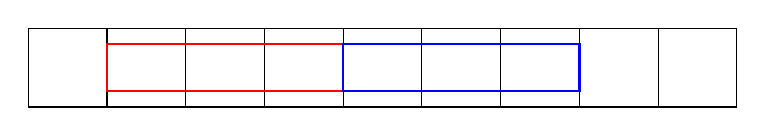
\begin{tikzpicture}
  % draw the array
  \foreach \x/\val in {0/1, 1/2, 2/3, 3/4, 4/5, 5/6, 6/7, 7/8, 8/9} {
    \draw (\x,0) rectangle ++(1,1) node[midway] {};
  }
  % draw the sliding window
  \foreach \x/\c in {1/red,4/blue} {
    \draw[thick,\c] (\x,0.2) rectangle ++(3,0.6);
  }
\end{tikzpicture}

于是,我们就可以这样不断地进行得到如下的代码:

\lstinputlisting[language=C++]{code/substring_with_concatenation_of_all_words.cpp}

\subsection{\href{https://leetcode.cn/problems/minimum-window-substring/}{最小覆盖子串}}

我们仍然需要去思考怎么去确定窗口的性质,我们首先定义一个变量\texttt{num}表示出现过多少个字符,当
\texttt{num}等于\texttt{t.size()}的时候,我们就找到了一个合法的子串。因此我们需要维持一个哈希表
表示在\texttt{windowStart}到\texttt{windowEnd}之间出现的字符的频率。由于我们需要找到最小的子串,
我们需要移动\texttt{windowStart},直到\texttt{num}不等于\texttt{t.size()}。关键就是后者的条件,
仅当我们遇到起作用的字符的时候,我们才需要停止移动\texttt{windowStart}。同时我们需要思考修不修改
\texttt{num}。

\lstinputlisting[language=C++]{code/minimum_window_substring.cpp}

\section{反转字符串系列}

反转字符串也是典型的双指针应用。

\subsection{\href{https://leetcode.cn/problems/reverse-string/}{反转字符串}}

这个题过于简单了,但是确实反转字符串的基础。我们可以使用两个指针,一个指向头,一个指向尾,然后
交换两个指针指向的元素,然后移动两个指针即可。

\lstinputlisting[language=C++]{code/reverse_string.cpp}

\begin{kaobox}[title=类似题目]
  \begin{itemize}
    \item \href{https://leetcode.cn/problems/reverse-vowels-of-a-string/}{反转字符串中的元音字母}
    \item \href{https://leetcode.cn/problems/reverse-string-ii/}{反转字符串 II}
    \item \href{https://leetcode.cn/problems/reverse-only-letters/}{仅仅反转字母}
  \end{itemize}
\end{kaobox}

\subsection{\href{https://leetcode-cn.com/problems/reverse-words-in-a-string/}{翻转字符串里的单词}}

一个最简单的思路就是函数式的做法,首先将字符串里面所有的单词抽取出来,然后反转,最后再拼接起来。但是这样会消耗极大的
空间,因为我们需要额外的空间来存储单词。我们可以使用双指针的方式来解决这个问题。我们如果首先对字符串进行翻转,我们
就可以得到单词的顺序是反的,然后我们再对每一个单词进行翻转,就可以得到我们想要的结果\sidenote{是不是一个十分聪明的
想法,然而并不是那么容易得出这个思路。}。

然而,这个问题还需要一个操作,需要对字符串的空格进行删除。这个过程仍然使用双指针的思路进行处理即可。

\lstinputlisting[language=C++]{code/reverse_words_in_a_string.cpp}

\end{document}
